\documentclass{article}
\usepackage{graphicx} % Required for inserting images
\usepackage{multicol}
\usepackage[shortlabels]{enumitem}
\usepackage{listings}
\usepackage{xcolor}
\usepackage{inconsolata}

\lstset{
    basicstyle=\ttfamily\color{red},
    language=C++,
}

\title{
    Algoritmos e Estrutura de Dados PCO001
    
    Resolução de: \textbf{Exercícios - Listas}
}
\author{Carlos Augusto Ribeiro}
\date{2024-01}

\begin{document}
    
\maketitle


\par
\noindent
\begin{center}
    \textbf{Instruções para execução da atividade:}
\end{center}
\begin{enumerate}[(a)]
    \item Para todos os exercícios propostos utilizar as implementações baseadas em \textbf{ponteiros}.
    \item Caso seja necessário, altere o tipo do dado a ser utilizado (e.g., \textbf{char} para \textbf{int}).
    \item A função implementada em uma tarefa pose ser utilizada na solução de outra (e.g., utilizar TamanhoLista para calcular a média dos valores de uma lista).
\end{enumerate}

\par
\noindent
\textbf{Tarefa 1} - Implemente uma função que verifica se um dado elemento inteiro pertence ou não a lista.
Protótipo: bool MembroLista (NoPtr, int).

\bigskip
\par
\noindent
\textbf{Solução}
\begin{lstlisting}
bool MembroLista(NoPtr no, int target) {
    if (no == nullptr) return false;
    if (no->Info == target) return true;
    return MembroLista(no->Lig, target);
}
\end{lstlisting}

\bigskip

\par
\noindent
\textbf{Tarefa 2}  - Implemente uma função para retornar o último elemento de uma lista.
Protótipo: NoPtr UltimoDaLista (NoPtr).

\bigskip
\par
\noindent
\textbf{Solução}
\begin{lstlisting}
NoPtr UltimoDaLista(NoPtr no) {
    if (no->Lig == nullptr) return no;
    return UltimoDaLista(no->Lig);
}
\end{lstlisting}

\bigskip

\par
\noindent
\textbf{Tarefa 3}  - Implemente uma função para retornar o número de elementos em uma lista.
Protótipo: int TamanhoLista (NoPtr).

\bigskip
\par
\noindent
\textbf{Solução}
\begin{lstlisting}
int TamanhoLista(NoPtr no) {
    if (no == nullptr) return 0;
    return TamanhoLista(no->Lig) + 1;
}
\end{lstlisting}

\bigskip

\par
\noindent
\textbf{Tarefa 4}  - Implemente uma função para retornar a média dos elementos de uma lista.
Protótipo: float MediaLista (NoPtr).

\bigskip
\par
\noindent
\textbf{Solução}
\begin{lstlisting}
float MediaLista(NoPtr no) {
    NoPtr aux = no;
    float soma = 0;
    while (aux != nullptr) {
        soma += aux->Info;
        aux = aux->Lig;
    }
    return soma / TamanhoLista(no);
}
\end{lstlisting}

\bigskip

\par
\noindent
\textbf{Tarefa 5} - Implemente uma função que retorna se duas listas são iguais ou não. Para serem consideradas iguais as listas precisam ter os mesmos elementos e ter o mesmo tamanho. A Figura 1 apresenta um exemplo do funcionamento dessa função.
Protótipo: bool ListasIguais (NoPtr, NoPtr).

\begin{figure}[h!]
	\clearpage
	\centering
	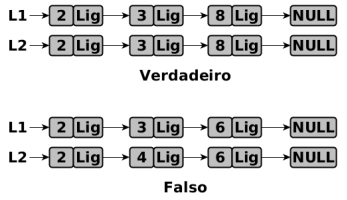
\includegraphics[width=0.6\linewidth]{lista/1.PNG}
	\caption{Exemplo do funcionamento da função ListasIguais.}
\end{figure}

\bigskip
\par
\noindent
\textbf{Solução}
\begin{lstlisting}
bool ListasIguais(NoPtr l1, NoPtr l2) {
    if (l1 == nullptr && l2 != nullptr) return false;
    if (l2 == nullptr && l1 != nullptr) return false;
    if (l1 == nullptr && l2 == nullptr) return true;
    if (l1->Info != l2->Info) return false;
    return ListasIguais(l1->Lig, l2->Lig);
}
\end{lstlisting}

\bigskip

\par
\noindent
\textbf{Tarefa 6}   - Implemente uma função que unifica (merge) duas listas em uma nova lista. A Figura 2 apresenta um exemplo do funcionamento dessa função.
Protótipo: NoPtr MergeListas (NoPtr, NoPtr).

\begin{figure}[h!]
	\clearpage
	\centering
	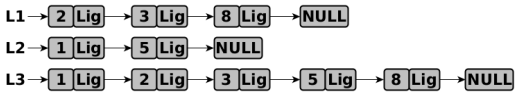
\includegraphics[width=0.8\linewidth]{lista/2.PNG}
	\caption{Exemplo do funcionamento da função MergeListas.}
\end{figure}

\bigskip
\par
\noindent
\textbf{Solução}
\begin{lstlisting}
NoPtr MergeListas(NoPtr l1, NoPtr l2) {
    NoPtr novaLista = nullptr;
    NoPtr aux = l1;
    while (aux != nullptr) {
        if (!MembroLista(novaLista, aux->Info))
        InsereLista(novaLista, aux->Info);
        aux = aux->Lig;
    }
    aux = l2;
    while (aux != nullptr) {
        if (!MembroLista(novaLista, aux->Info))
        InsereLista(novaLista, aux->Info);
        aux = aux->Lig;
    }
    return novaLista;
}
\end{lstlisting}

\bigskip    
\end{document}
